\documentclass[journal]{IEEEtran}
\usepackage{graphicx}
\usepackage{listings}	% For inserting code
\usepackage{minted}		% For inserting code
\setminted[systemverilog]{
	tabsize=3
}
\setminted[C]{
	tabsize=3
}
\usepackage{xspace}		% For using \SV with trailing spaces
\usepackage{cleveref}	% Needed for correctly referencing listings

\AtBeginEnvironment{minted}{%
  \renewcommand{\fcolorbox}[4][]{#4}}
\newcommand{\SV}{SystemVerilog\xspace}

\title{My thoughts on UVM, SystemVerilog and creating a like implementation in Chisel/Scala}
\author{Kasper Juul Hesse Rasmussen\\
s183735@student.dtu.dk\\
Technical University of Denmark
}
\begin{document}
\maketitle

\section{Introduction}
The purpose of this document is to outline my findings during the course of the Chisel-UVM project. It should serve as a reference on what the UVM can do, how it works, and how some of this (namely the SystemVerilog Direct Programming Interface (DPI)) may be implemented in a Scala based testing framework.

\section{UVM}
The Universal Verification Methodology (UVM) is a testing framework built on top of the testing capabilities of SystemVerilog. In that respect, there is nothing you can do in the UVM that you cannot also do in plain SystemVerilog. The main purpose of UVM was to standardize testing the testing framework used across EDA vendors, making it easier for users to use their testbenches across different software suites.

The testbench in the UVM is built up around two key components. The \textbf{scoreboard} and \textbf{coverage collector}. Together, these components check whether the DUT operates as expected, and whether the verification procedure can be thought to be finished.

\subsection{Scoreboard}
The purpose of the scoreboard is to ensure that the DUT matches specification. When using directed tests, this may be as simple as constructing a list of output values and checking these in order. When using randomized testing, the scoreboard is usually implemented as a software model (sometimes called a golden model) which is defined to be correct. The software model should mimic the functionality of the DUT, and thus provide the same outputs given the same inputs. 

The scoreboard may be implemented purely in SystemVerilog. Being a combined HDL and HVL, SystemVerilog supports procedural and object-oriented paradigms for testbench design. One of the benefits that \SV adds to the table is the ability to interface with C-code through the use of the \SV Direct Programming Interface (DPI). This is an interface which allows C code to be called from inside the \SV testbench, and likewise allows for \SV code to be called from inside of a C program. Programming low-level simulations of hardware is most likely easier in C than in plain \SV. In listing \ref{lst:dpi} is shown a simple example of some SystemVerilog code calling C code through the \SV DPI.

A scoreboard doesn't necessarily "rate"\, the performance of the DUT by comparing it to other modules, as one might expect from the name. A better name might simply be "checker". 

\begin{listing}[htbp]
\begin{minted}{C}
//hello.c
#include "svdpi.h"
#include <stdlib.h>

void c_hello(char* name) {
	printf("Hello from C, %s", name);
}
\end{minted}
\begin{minted}[breaklines]{systemverilog}

//hello.sv
module tb;
import "DPI-C" function void c_hello(string name);

	initial main();
	task main();
		c_hello("SystemVerilog");
	endtask
endmodule

// Outputs: "Hello from C, SystemVerilog"
\end{minted}
\caption{Short example showing how to use the \SV DPI to execute C-code from within \SV.}
\label{lst:dpi}
\end{listing}

\subsection{Constrained random verification}

Most UVM testbenches employ "Constrained Random Verification"\, (CRV) for generating test stimulus. This is as opposed to using directed testing, where input vectors are predefined to test a certain behaviour. With CRV, random test stimuli are generated. The "Constrained" part of CRV implies that these values aren't entirely random, but are chosen to fulfill a series of criteria. If eg. the DUT is an ALU with a 5-bit opcode field of which only 20 bit-patterns are used, it would be prudent to only generate the 20 valid opcodes for most test purposes. Specific tests could then be written to ensure proper operation if an invalid opcode was asserted.

An example of a class with randomized variables is seen in listing \ref{lst:crv}. The keyword \texttt{constraint} is used to constrain a variable defined with the \texttt{rand} keyword.

One randomized variable, \texttt{bcd}, is a 4-bit field which only takes on values in the range 0 and 9. The field \texttt{value} has a $1/3$ chance of being 0, $1/3$ of being 255 and $1/3$ of being any other value. The fields \texttt{a,b,c} must satisfy $0<a<b<c$. The field \texttt{op} has no constraints, and will thus randomly toggle between  0, 1, 2 and 3, the only values it can take on.

\begin{listing}[htbp]
\begin{minted}{systemverilog}
//Myclass.svh
class Myclass;
rand logic [3:0] bcd;
rand logic [7:0] value;
rand logic [3:0] a, b, c;
rand logic [1:0] op;

constraint c_BCD {
	bcd inside {[0:9]};
}
constraint c_value {
	value dist {
		0:/1,
		[1:254]:/1,
		255:/1
	};
}
constraint c_abc {
	0 < a;
	a < b;
	b < c;
}
// op isn't constrained, but is randomized
endclass: Myclass
\end{minted}
\caption{Example SystemVerilog code showing how different values are constrained.}
\label{lst:crv}
\end{listing}

In listing \ref{lst:usingcrv}, an object of type \texttt{Myclass} is instantiated and randomized using the \texttt{mc.randomize()} command. Finally, the \SV function \texttt{\$display} is used to print the value of the BCD field.

\begin{listing}[htbp]
\begin{minted}{systemverilog}
//top.sv
`include "Myclass.svh"
module top;
  Myclass mc;
  initial begin;
    mc = new;
    mc.randomize();
	 $display(mc.bcd);
  end
endmodule
\end{minted}
\caption{Example SystemVerilog code showing how to instantiate and randomize a class with random fields.}
\label{lst:usingcrv}
\end{listing}

\subsection{Coverage collection}
The purpose of coverage collection is to check whether all "interesting"\, (as defined by the verification engineer) input combinations have been generated. For the ALU mentioned above, it might be interesting to check whether all opcodes work correctly when asserted after a reset, and whether over/underflow flags are correctly set when performing arithmetic operations. 

An example of coverage collection is seen in listing \ref{lst:cov} where the randomized values from before are covered. A \textit{covergroup} is a label used to collect relevant values under the same heading. A \textit{coverpoint} is a directive instructing the simulator that the given value should be monitored for changes. In the declaration of the coverpoint, several \textit{bins} are generated. These bins correspond to the bins of a histogram. Every time an event occurs which matches the declaration inside a bin, the counter associated with that bin is incremented by one. An event may cause multiple bins to increment at the same time.

\begin{listing}[htbp]
\inputminted{systemverilog}{snippets/Cover.svh}
\caption{Examle SystemVerilog code showing how covergrups and coverpoints are organized.}
\label{lst:cov}
\end{listing}

In the coverage declarations shown in listing \ref{lst:cov}, the covergroup \texttt{cg\_bcd} only covers one field, \texttt{bcd}. The bin is labeled by prepepending \texttt{BCD:} in front of the name. 10 bins are generated which each sample the values 0-9, and the remaining values 10-15 are sampled into the default bin \texttt{others}. 

In the covergroup \texttt{cg\_others} three coverpoints are set up. The \texttt{VAL} coverpoint only explicitly samples 3 ranges of values. The \texttt{A} coverpoint auto-generates one bin for each possible value it may take on, 16 bins in total, since no bins are explicitly declared. The coverpoint \texttt{OP} has one bin, \texttt{toggle} which only increments when \texttt{mode} toggles from \texttt{0x0} to \texttt{0x1}. Finally, the \texttt{cross} statement implements cross coverage. Cross coverage tracks what values were sampled at multiple coverpoints at the same time.

Using the cross of \texttt{A} and \texttt{OP}, it may be possible to have 100\% coverage on both coverpoints (ie. all bins have been hit at least once), but the cross coverage may not be at 100\% if eg. \texttt{OP} never toggled while \texttt{A} was 1. Increasing the number of random samples that are generated may alleviate this problem. If it doesn't, it may be indicative that something is wrong in the structure of the testbench or DUT.

In listing \ref{lst:usingcov}, the module from \cref{lst:usingcrv} has been expanded to also use the coverage collector.
\begin{listing}
	\inputminted{systemverilog}{snippets/top.sv}
	\caption{Showcasing how multiple random values are generated and sampled by the coverage collector.}
	\label{lst:usingcov}
\end{listing}

In figure xx, the result of running the 20 iterations is seen for coverpoints \texttt{BCD, A, VAL}. 

\begin{figure}
	\centering
	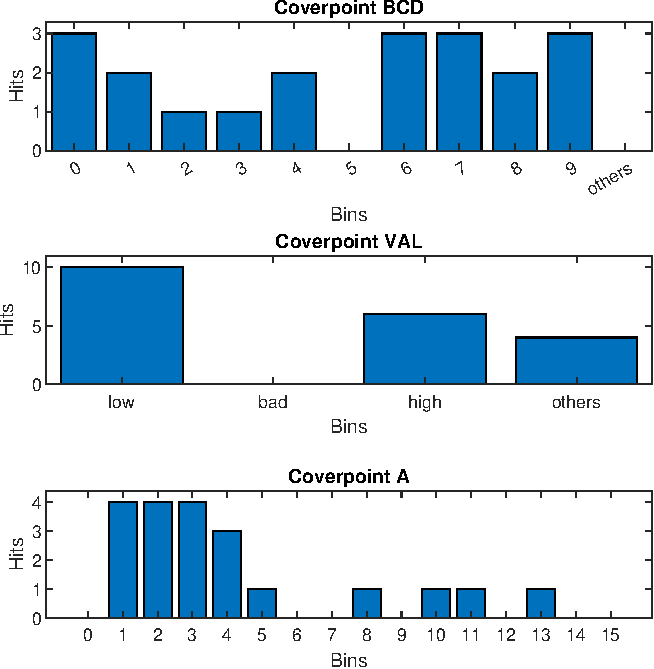
\includegraphics[width=\columnwidth]{coverage.pdf}
\end{figure}
\end{document}

% *Explain what CRV is
% *Explain what coverage is, how it works
% *Show an example of a coverage histogram.
% TODO Explain the basics of UVM testbenches
% TODO Explain how the SV DPI works
% Explain how the java JNI works
% Collect it all together